Our recommendations prioritize security by design principles. Because most of the home IoT users lack the technical knowledge or awareness to set up a secured system, the underlying architecture of IoT protocols and the default settings should be secure, and set to alert users to vulnerabilities. Such settings benefit downstream developers with little to no experience in cybersecurity as they build IoT products and applications. As noted earlier, even though some of our recommendations are Zigbee-specific, we believe other protocols should also pay attention to same considerations as they design similar protocols.

We assess the key security and privacy concepts on a maturity scale below, followed by detailed assessment of each concept and our recommended steps.

\begin{figure}[h]
	\caption{Maturity Scale}
	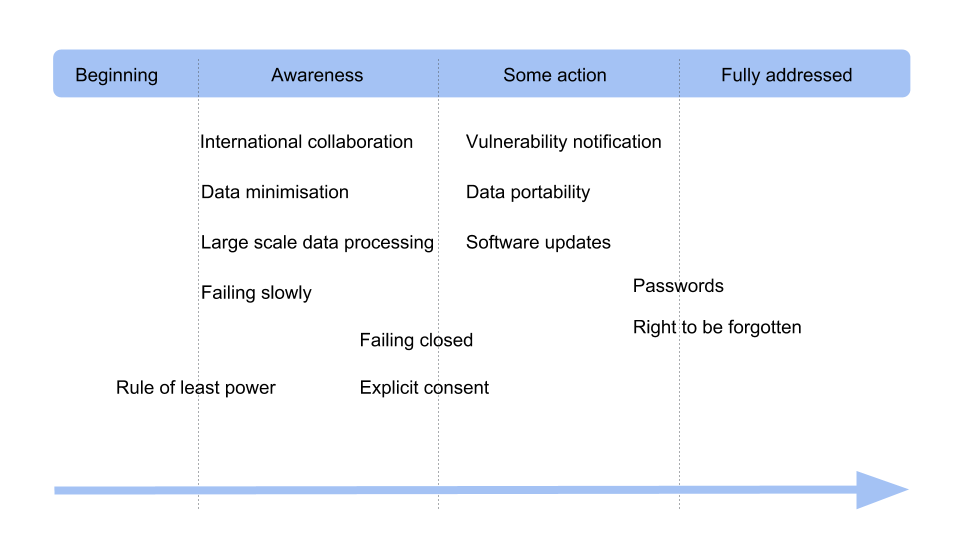
\includegraphics[width=1.0\textwidth]{table}
\end{figure}

\subsection{Concepts with Some Reflection in Policy}

\subsubsection{Preventing Weak and Default Passwords}
Easily guessable passwords are a rational concern in the home automation threat model because they allow for the sorts of automated attacks that are common in practice. Usage of weak or hardcoded default passwords can be prevented by a combination of policy and technical measures.

\noindent{\bf Technology:}  IoT protocols can contribute to enforcing good password practices by centralizing authentication to a “hub” device. In the case of Zigbee, since there already exists a Zigbee Trust Center in every node, IoT devices should defer login and authentication to said node, rather than authenticating the user at the device’s own application layer akin to an authentication proxy. The Zigbee Trust Center can thus enforce good password practices, including but not limited to enforcing non-default passwords, and making a call to Troy Hunt’s haveibeenpwned database and service, that checks for poor password practices as well as whether the credentials being registered have been leaked before (“Pwned Passwords in Practice,” 2018).

\noindent{\bf Policy:} Default passwords are a good candidate for policy mitigation because their presence is definite; that is, unlike a security flaw such as a subtle error in source code or an incorrectly implemented encryption protocol, it is reasonable to expect manufacturers to be able to guarantee that a weak default password is not present. 

\noindent{\bf Current Policy Measures:} The IoT Cybersecurity Act mandates that IoT devices sold to the federal government not include “fixed or hard-coded credentials”. While it does not apply to non-government purchases, it could serve as a bellwether for the feasibility of a more general policy. In addition, the Code of Practice for IoT Security, a non-binding guideline issued by the UK Department for Culture, Media, and Sport, recommends that “[a]ll IoT device passwords shall be unique and not resettable to any universal factory default value.” 

\noindent{\bf Our recommendations:}
\begin{enumerate}
\item Wider adoption of the sample password regulations,
\item Enforcement of good passwords through the Zigbee consortium
\end{enumerate}



\subsubsection{Software Updates and Vulnerability Notification}
Software updates are a practical approach to improving home automation security as they enable periodic fixes to the known flaws often exploited by malware. While it is possible that a user could be attacked with a previously-unknown exploit, once an exploit is used by malware “in the wild”, it should be possible for the manufacturer to determine what bug is being exploited and patch it. We recommend a combination of policy and technical measures to encourage regular software updates.

\noindent{\bf Technology:} While some IoT platforms have automated vulnerability patching (e.g. Ubuntu Core), automated vulnerability patching - or at least, notification - should be a core functionality of any protocols including Zigbee. Since every Zigbee Network Coordinator registers new IoT devices, connecting IoT devices can send an additional data packet containing a hashed version number of the firmware and software running on it. Zigbee Network Coordinators can store an additional field in its internal record of connected devices to include version numbers, and on a regular basis ping a service managed by the Zigbee Consortium that contains the latest firmware and software version hashes to compare if the local IoT devices’ version hashes match that of the latest version. Since the Zigbee Consortium requires any new products developed to be registered with them, they would be able to maintain a centralized database of firmware and software version numbers, and mandate developers to keep this database up-to-date. The Zigbee Network Coordinator would then be able to automatically instruct IoT devices on the network to update should they fail the check, or warn the user to apply the update if a human is required. Such version checking would also allow the Zigbee Network Coordinator to warn the user if there are active vulnerabilities on the devices.

\noindent{\bf Current Policy Measures:} The Code of Practice for IoT Security specifies that devices should be either easily updatable or easily replaceable, that the importance of updating should be made clear to consumers, and that the duration of time for which a product will be supported with new updates should be made clear. The IoT Consumer TIPS Act of 2017 directs the FTC to develop educational materials for users of IoT devices and specifies that such materials should cover updating software. Neither policy can guarantee that educational materials will actually make their way to every consumer, or who will then apply them. However, educating consumers on how and why to update devices is a good first step. Taking it a step further, the US Department of Homeland Security’s report on “Strategic Principles for Securing the Internet of Things” recommends automated patching of IoT device, which if made into policy, would be a big step to combating the long tail of unpatched devices (“Strategic Principles for Securing the Internet of Things (IoT),” 2016).

On the vulnerability notification side, we see industry leaders supporting this principle; for example, disclosure requirements were recently highlighted as a key action item by Google’s Framework for Responsible Data Protection Regulation (Enright, 2018). Transparency requirement can be seen as an alternative solution to the fact that no tamper-proof technology is available and transparency is the first step for the IoT community to do a better job in identifying problems and addressing them effectively.

\noindent{\bf Our Recommendations:}
Automated vulnerability patching to be encouraged by both technical consortia and policy makers.

\subsection{Concepts for Encouraging Security-by-Design}

\subsubsection{Failing Closed}

The concept of failing closed versus failing open in a system design comes from the question that arises around what systems and applications should do when an error or exception to the expected behavior occurs. By definition, systems that fail open allow access or continue to operate, while systems that fail closed deny access or ceases to function (“Security Fundamentals Part 1: Fail Open vs. Fail Closed” 2014). Login pages on many internet websites, such as Amazon or banks, are a good example of this - attempting to log on with the wrong password to an account too many times results in a freeze on further login attempts for a time period, as well as sending a notification via email or text message to the owner.

\noindent{\bf Technology:} In the context of smart home devices, failing closed prioritizes security over function, and users are more likely to be aware of the existence of a security or privacy issue if one of their smart home devices ceases to function as a result (O’Haver, 2016). There are many ways that home IoT systems can fail closed, and this relies on some security-minded sensibilities on the side of the developer. For example, an IP camera can cease to function and send an alert to the owner the moment an unauthorized user is detected accessing the camera’s live feed - in this instance, the owner’s privacy is protected by a fail closed design, rather than letting an unauthorized user spy on them. A smart stovetop can shut off if it detects an unauthorized user attempting to turn on the burner without any authorized users in its vicinity, potentially preventing a fire from starting.

While a number of fail closed designs may result in the occasional inconvenience towards the user due a device ceasing to operate, this would encourage users to set up properly configure their devices and would result in stronger long-term security. Furthermore, we believe that a larger shift towards this school of thought would result in the inconvenience becoming “invisible”, much like how very little second thought is given to locking the front door after an individual leaves their house.

\noindent{\bf Policy:} This concept exists primarily in the systems design and cybersecurity domains, and as a result, nothing stood out in our analysis explicitly addressing this issue.

\noindent{\bf Our Recommendations:} We recommend that Zigbee incorporates failing closed in the protocol design, especially when taking actions that are inherently dangerous, like recognizing a new trusted device. 

\subsubsection{Failing Slowly}
Failing slowly is related to failing closed in that it leverages the communications that must occur before triggering a dangerous command to give the user the chance to correct course. However, it can have less impact on usability, which in consumer devices might mean the difference between easy access and a safe home.


\noindent{\bf Technology:} There are several protocols that result in slower decision making, and the developer must choose which fits based on the specific user and adversaries expected. Options include:
\begin{enumerate}
\item A protocol that consists of several re-confirmations on the part of the user. This is the least convenient method but notifies the user so that they can prevent a dangerous action.
\item A protocol that adds a significant wait time before triggering a command. While the user does not need to reengage to achieve the desired outcome the adversary is forced to maintain control for a longer period of time, which limits attack automation.
\item A protocol that adds a random amount of time before triggering a command. This has the least impact on users but addresses adversaries who intend to use a botnet since it makes devices harder to synchronize actions.
\end{enumerate}


\noindent{\bf Policy:} Nothing stood out in our analysis explicitly addressing this issue.


\noindent{\bf Our Recommendations:}
Zigbee should add the three protocols above to the network layer API so that developers who want to fail slowly have correctly implemented code and developers who were not considering failing slowly might be nudged towards this valuable design concept.

\subsection{Concepts that Give Developers Secure Tools}
\subsubsection{Forward Security}
Forward secrecy protects consumers from adversaries who store information transmitted over long periods of time: without forward secrecy learning a single key revels the whole data set, but with forward secrecy only a subset is revealed. 


\noindent{\bf Technology:} Facebook Messenger and Whatsapp all use a protocol called Signal that provides forward secrecy, but other companies have been slow to adopt it given the complexity of the algorithm. 


\noindent{\bf Policy:} Nothing stood out in our analysis explicitly addressing this issue but could be a valuable way to decrease the negative impact of mass data dumps during attacks.


\noindent{\bf Our Recommendations:} Zigbee should include a correct implementation of the Signal protocol along with the encryption primitives that are already provided.

\subsubsection{Rule of Least Power}
The rule of least power states that a system should be built the least powerful language that can accomplish the system’s task. “Language power” can be thought of as the freedom that a developer is given. In a language like C developers have direct control over the computer’s memory, but in a language like Rust the compiler handles memory. There are tradeoffs: while computers are very well suited to the kind of bookkeeping that Rust does, the freedom that comes with C allows developers to make programs that are more time and space efficient.


\noindent{\bf Technology:} Ultimately, languages that are easy to reason about and address the types of errors that computers are simply better at catching encourage more secure implementations. State machines are often used as visual aids in the design phase of product development and constitute a sub-Turing-complete\footnote{A well-defined marker of language limitation} language.

\noindent{\bf Policy:} Nothing stood out that explicitly addresses this issue in our analysis.


\noindent{\bf Our Recommendations:} Define a finite state machine language in the application layer that requires developers to define input and output formats. Transitions between states can be based on timer expirations, sensor results, interrupts, or send commands to actuators and nothing else. Given that information it is possible to generate the code needed for the application. The compiler could also provide a graphic of the defined state machine in order to give clearer feedback (this takes advantage of another valuable side effect of low-power languages: information resuse). While we believe the application layer should continue to provide the high power language it currently does, a lower power language of state machines might be intuitive enough to encourage developers to leave the bookkeeping to the computers.


\subsection{Concepts that Policy Makers are Encouraging}
While the following three recommendations cannot be tied into the Zigbee protocol, they are an important part of the landscape for protocol designers, device developers, and consumers. The specific policies highlighted are not necessarily designed for the internet of things specifically, but we believe they are relevant to home automation security given our threat model.

\subsubsection{Explicit Consent}
A hazard of IoT is the harvesting of user data in a way that may be intentional on the part of device manufacturers, but is against the desires of the user. We believe this issue is sufficiently addressed by recent policies.

\noindent{\bf Policy:} This issue is extensively addressed by recent regulations. The California Consumer Privacy Act and the EU General Data Protection Regulation attempt to mitigate this by requiring companies to clearly disclose what information is being collected and allow the user to prevent information from being shared or sold. While some details are left to technical implementation, these policies establish the basic rights and expectations of consumers. 

\noindent{\bf Our Recommendations:} Wider adoption of explicit, opt-in consent of users for data collection.


\subsubsection{Data Minimization}
In the Home IoT context, data minimization requirement would limit data hoarding by installed devices which is an important requirement to preserve consumer privacy and leads to less exposure in case of a security breach. We believe action from policy makers can lead companies to adopt data minimization measures. 

\noindent{\bf Policy:} GDPR has been the leading regulation in the push for limiting the amount of data being collected by companies while also limiting the use of data for purposes other than disclosed to the consumer at time of collection (Dataguise, 2017). This policy push stands against the current practices of many companies that prioritize data hoarding, mainly for marketing purposes and also with the hope that new technologies will enable leveraging of more granular data in the future (Woodie, 2016).

\noindent{\bf Our Recommendations:} Policy makers should push for data minimization in order to protect their consumers’ right to privacy. 

\subsubsection{International Collaboration}
Governments are increasingly paying attention to cybersecurity issues as an international concern that requires collaboration to effectively tackle. This awareness can be encouraged by all stakeholders in IoT to come up with international guidelines and frameworks.

\noindent{\bf Policy:} While the EU is taking a relatively more international approach in regulating technologies for privacy and security preservation purposes, most countries tend to set nation-level (state level in the US example) standards and policies to address these concerns. Guidelines such as National Institute of Standards and Technology (NIST)’s cybersecurity framework can help develop a common language and a basis for international collaboration, which becomes more crucial to address cyber attacks effectively (Waldron 2017).

\noindent{\bf Our Recommendations:} Further push by all stakeholders to foster international collaboration.
